The Component Library is a function inspired by the SUAS Reference Architecture \citep{Jacques2019}. The goal is to have a library of components to choose from for each subsystem for rapid prototyping that improves over time. As teams create new CubeSat designs, the individual components can be stored in the Component Library for future reuse by other teams. For example, if there are multiple commercially available solar arrays that previous teams have used in their designs, those solar arrays will be available to reuse with all of their value properties already filled in. A team could swap out multiple solar arrays from the Component Library in their EPS subsystem diagram and perform analysis to quickly assess how each one performs for their system. Figure \ref{fig:Component Library} shows the top level view of the Component Library, which has a separate package for each subsystem. 

Figure \ref{fig:CL Structures} shows how it could be used in a simple example with different CubeSat bus sizes. In the Structures package, multiple chassis sizes, with their dimensions all filled out, can be quickly copied and pasted into a new model. If some value differs from the default values provided, the team would just need to make those modifications. Figure \ref{fig:CL EPS} shows how Enumeration lists are also stored in the component library to be used throughout the model. These enumeration lists are all consolidated in their respective subsystem packages instead of scattered across the physical model. In this example, instead of typing in a string of text to denote the battery chemistry, the user can just select from a drop-down list of the available types in the enumeration list. These are created for many subsystems, and as new choices become available, these can be updated. 

\begin{figure}[H]
    \centering
    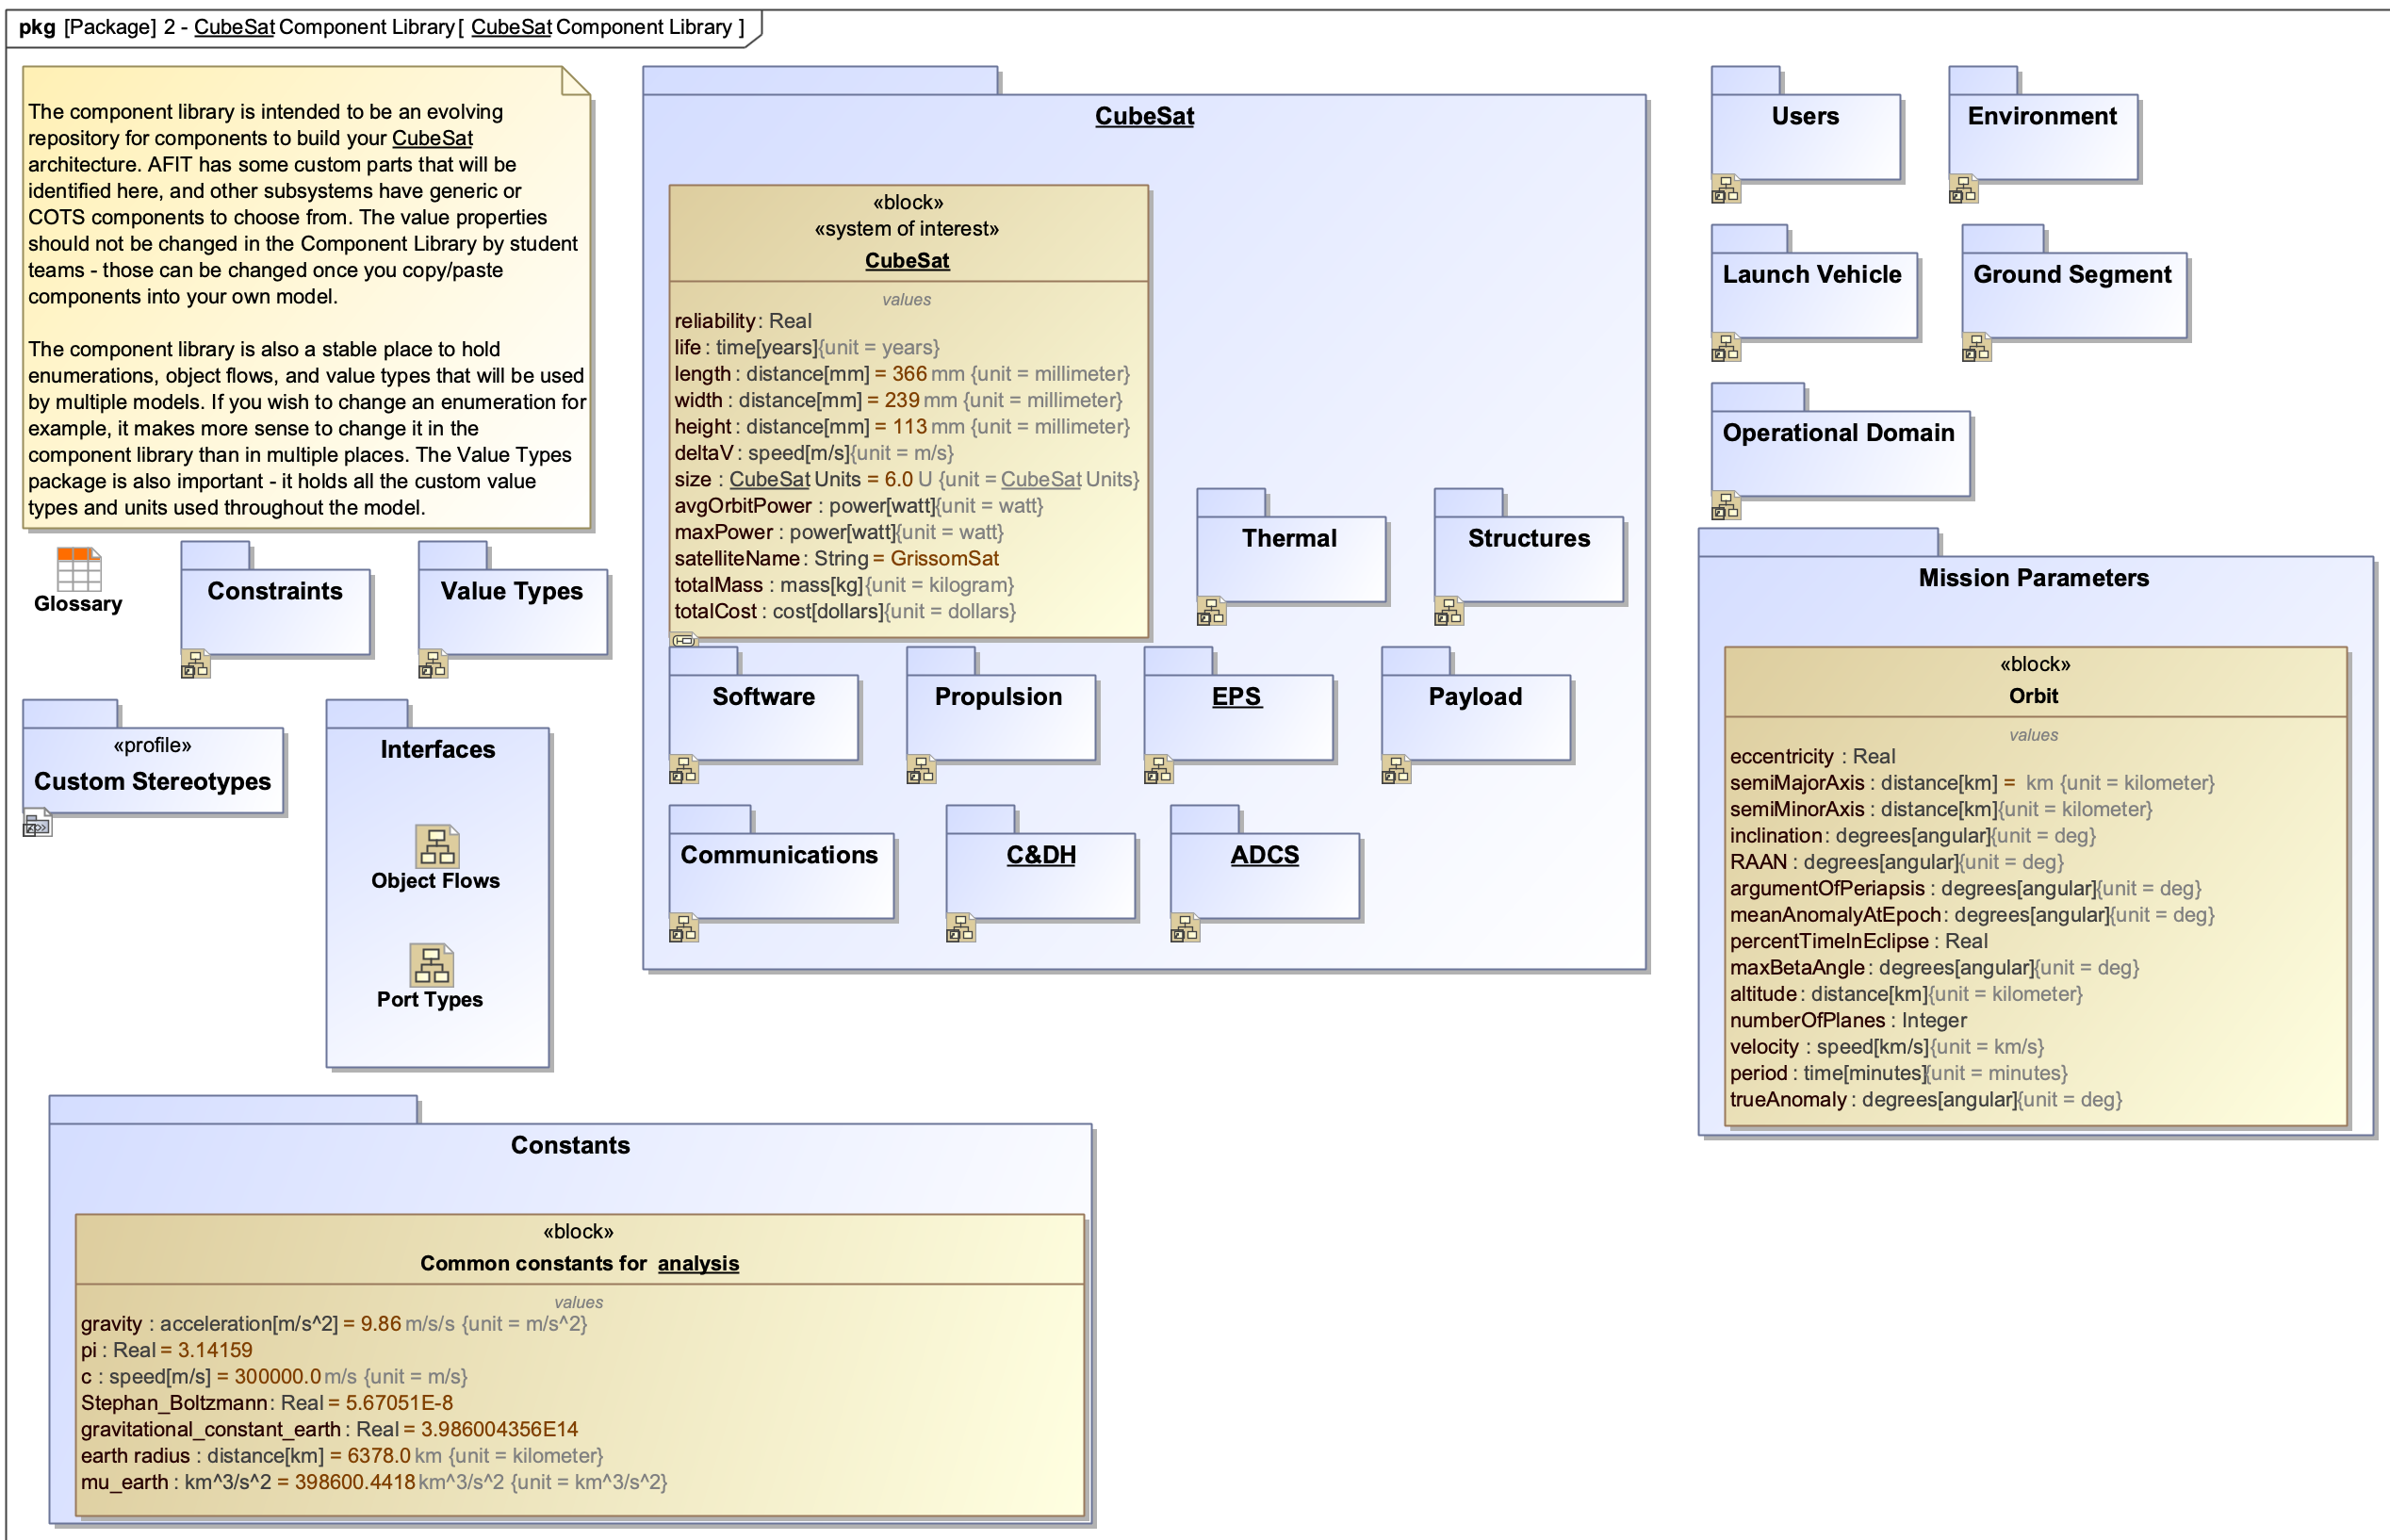
\includegraphics[width=\textwidth]{Thesis/Analysis_and_Results/Analysis and Results Figures/Component Library.png}
    \caption{Component Library}
    \label{fig:Component Library}
\end{figure}

\begin{figure}[H]
    \centering
    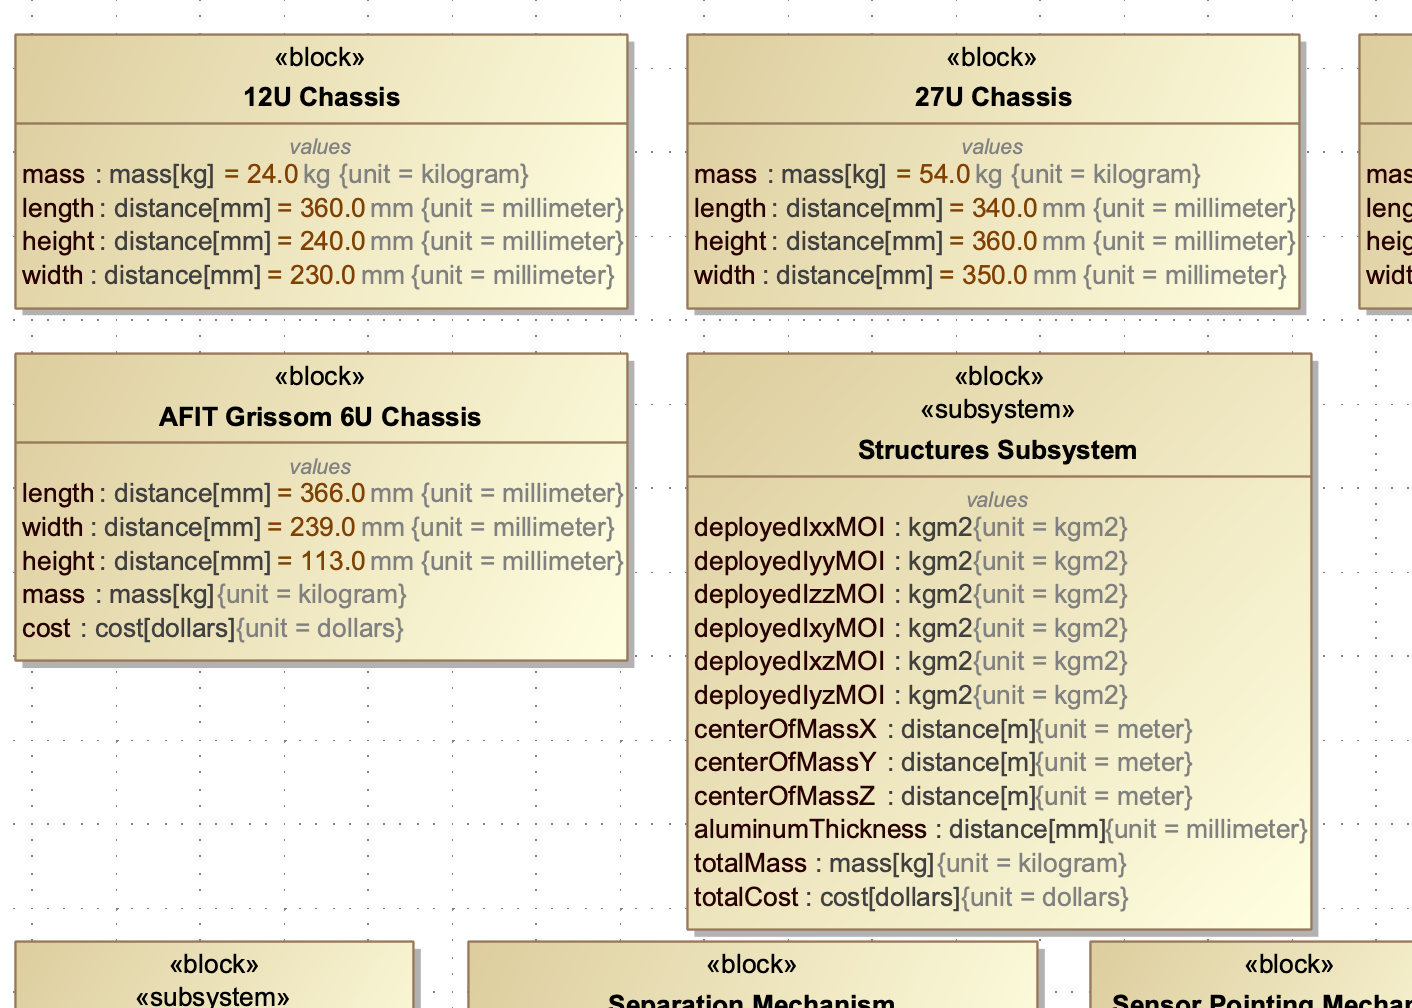
\includegraphics[width=4 in]{Thesis/Analysis_and_Results/Analysis and Results Figures/CL Structures.png}
    \caption{Component Library - Structures}
    \label{fig:CL Structures}
\end{figure}

\begin{figure}[H]
    \centering
    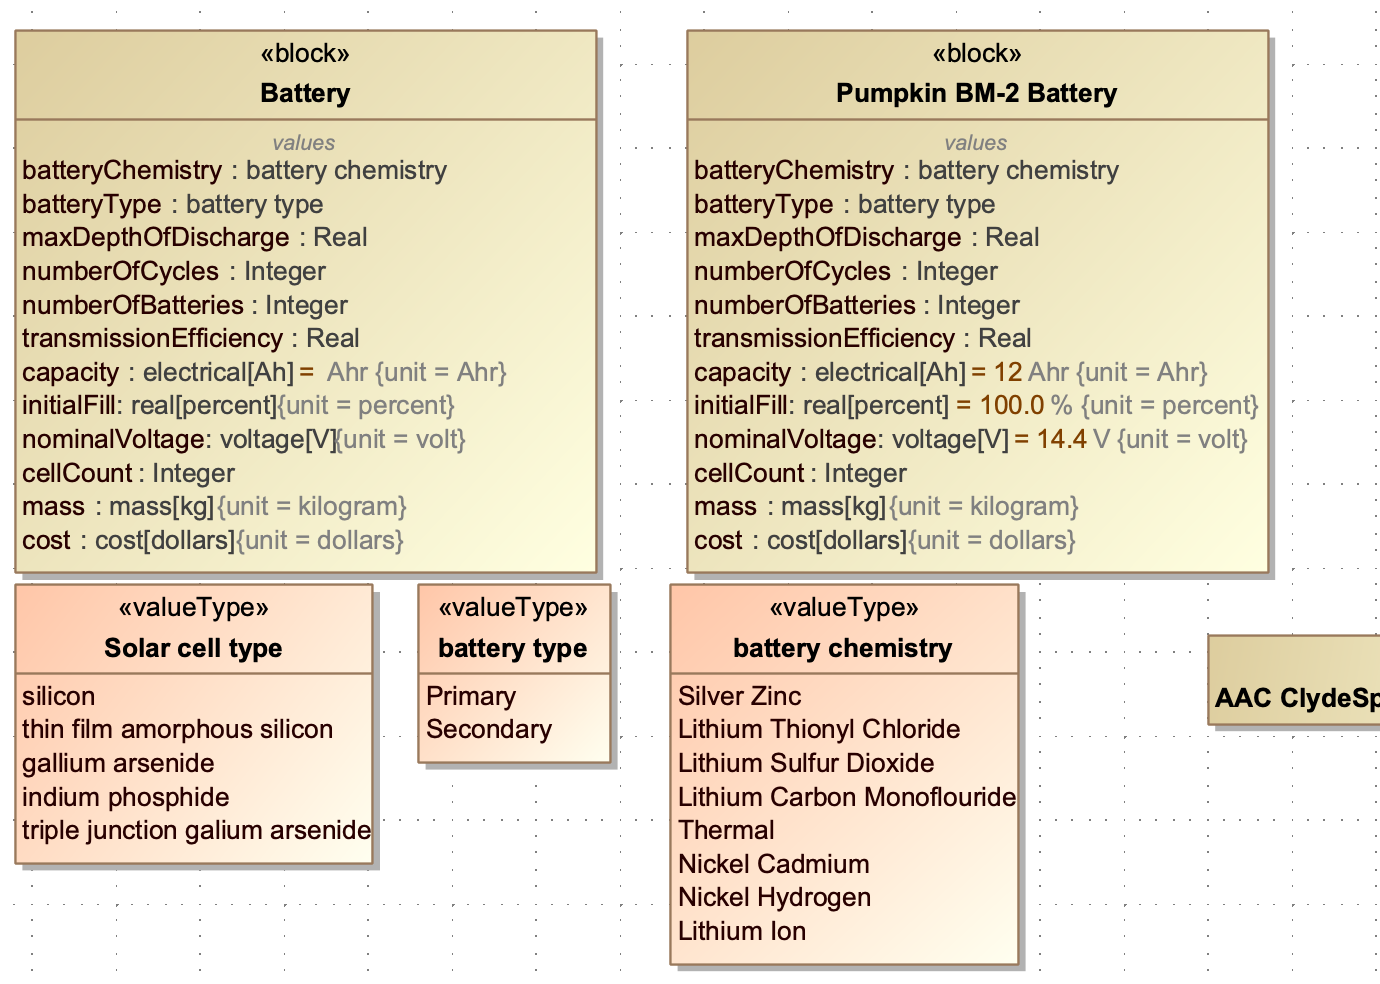
\includegraphics[width=4 in]{Thesis/Analysis_and_Results/Analysis and Results Figures/CL EPS.png}
    \caption{Component Library - EPS}
    \label{fig:CL EPS}
\end{figure}

Another important area of the Component Library is the custom Value Type library. Using the default ISO-8000 library seemed like the logical choice for units, but there were several issues with it that caused frustration over time. Most value types in the ISO-8000 library were never used and crowded the selection window when a user would try to find a unit, the spelling and naming conventions did not match what students were expecting or were accustomed to, and most importantly, they were not able to be modified without causing errors every time Cameo was opened. To alleviate these issues, an entire custom value type library was created to stay more organized and allow for easy modifications and customization. The Value Types, Units, and "QuantityKinds" (a SysML necessity for units to work properly in analysis) are all stored neatly in packages based off their type. When a user is going to add a new Value Property to a component block, it is now very easy to find the relevant value type to assign to it. The default practice amongst students without having this central repository is to just type in a new Value Type, and then that Value Type appears in the same location as that block. This isn't necessarily a bad thing on a small model, but a Reference Architecture is meant to be used for multiple candidate architectures and multiple projects, and referencing a new Value Type that belongs to another physical model should be avoided. For that reason, all Value Types are stored in one central place within the Component Library. This has also been done with Object Flows in the Reference Architecture. Object Flows represent the flow of objects, whether they are matter, energy, or data, primarily used in the Mission Context diagram shown earlier in Figure \ref{fig:Mission Context ibd}.

\begin{figure}[H]
    \centering
    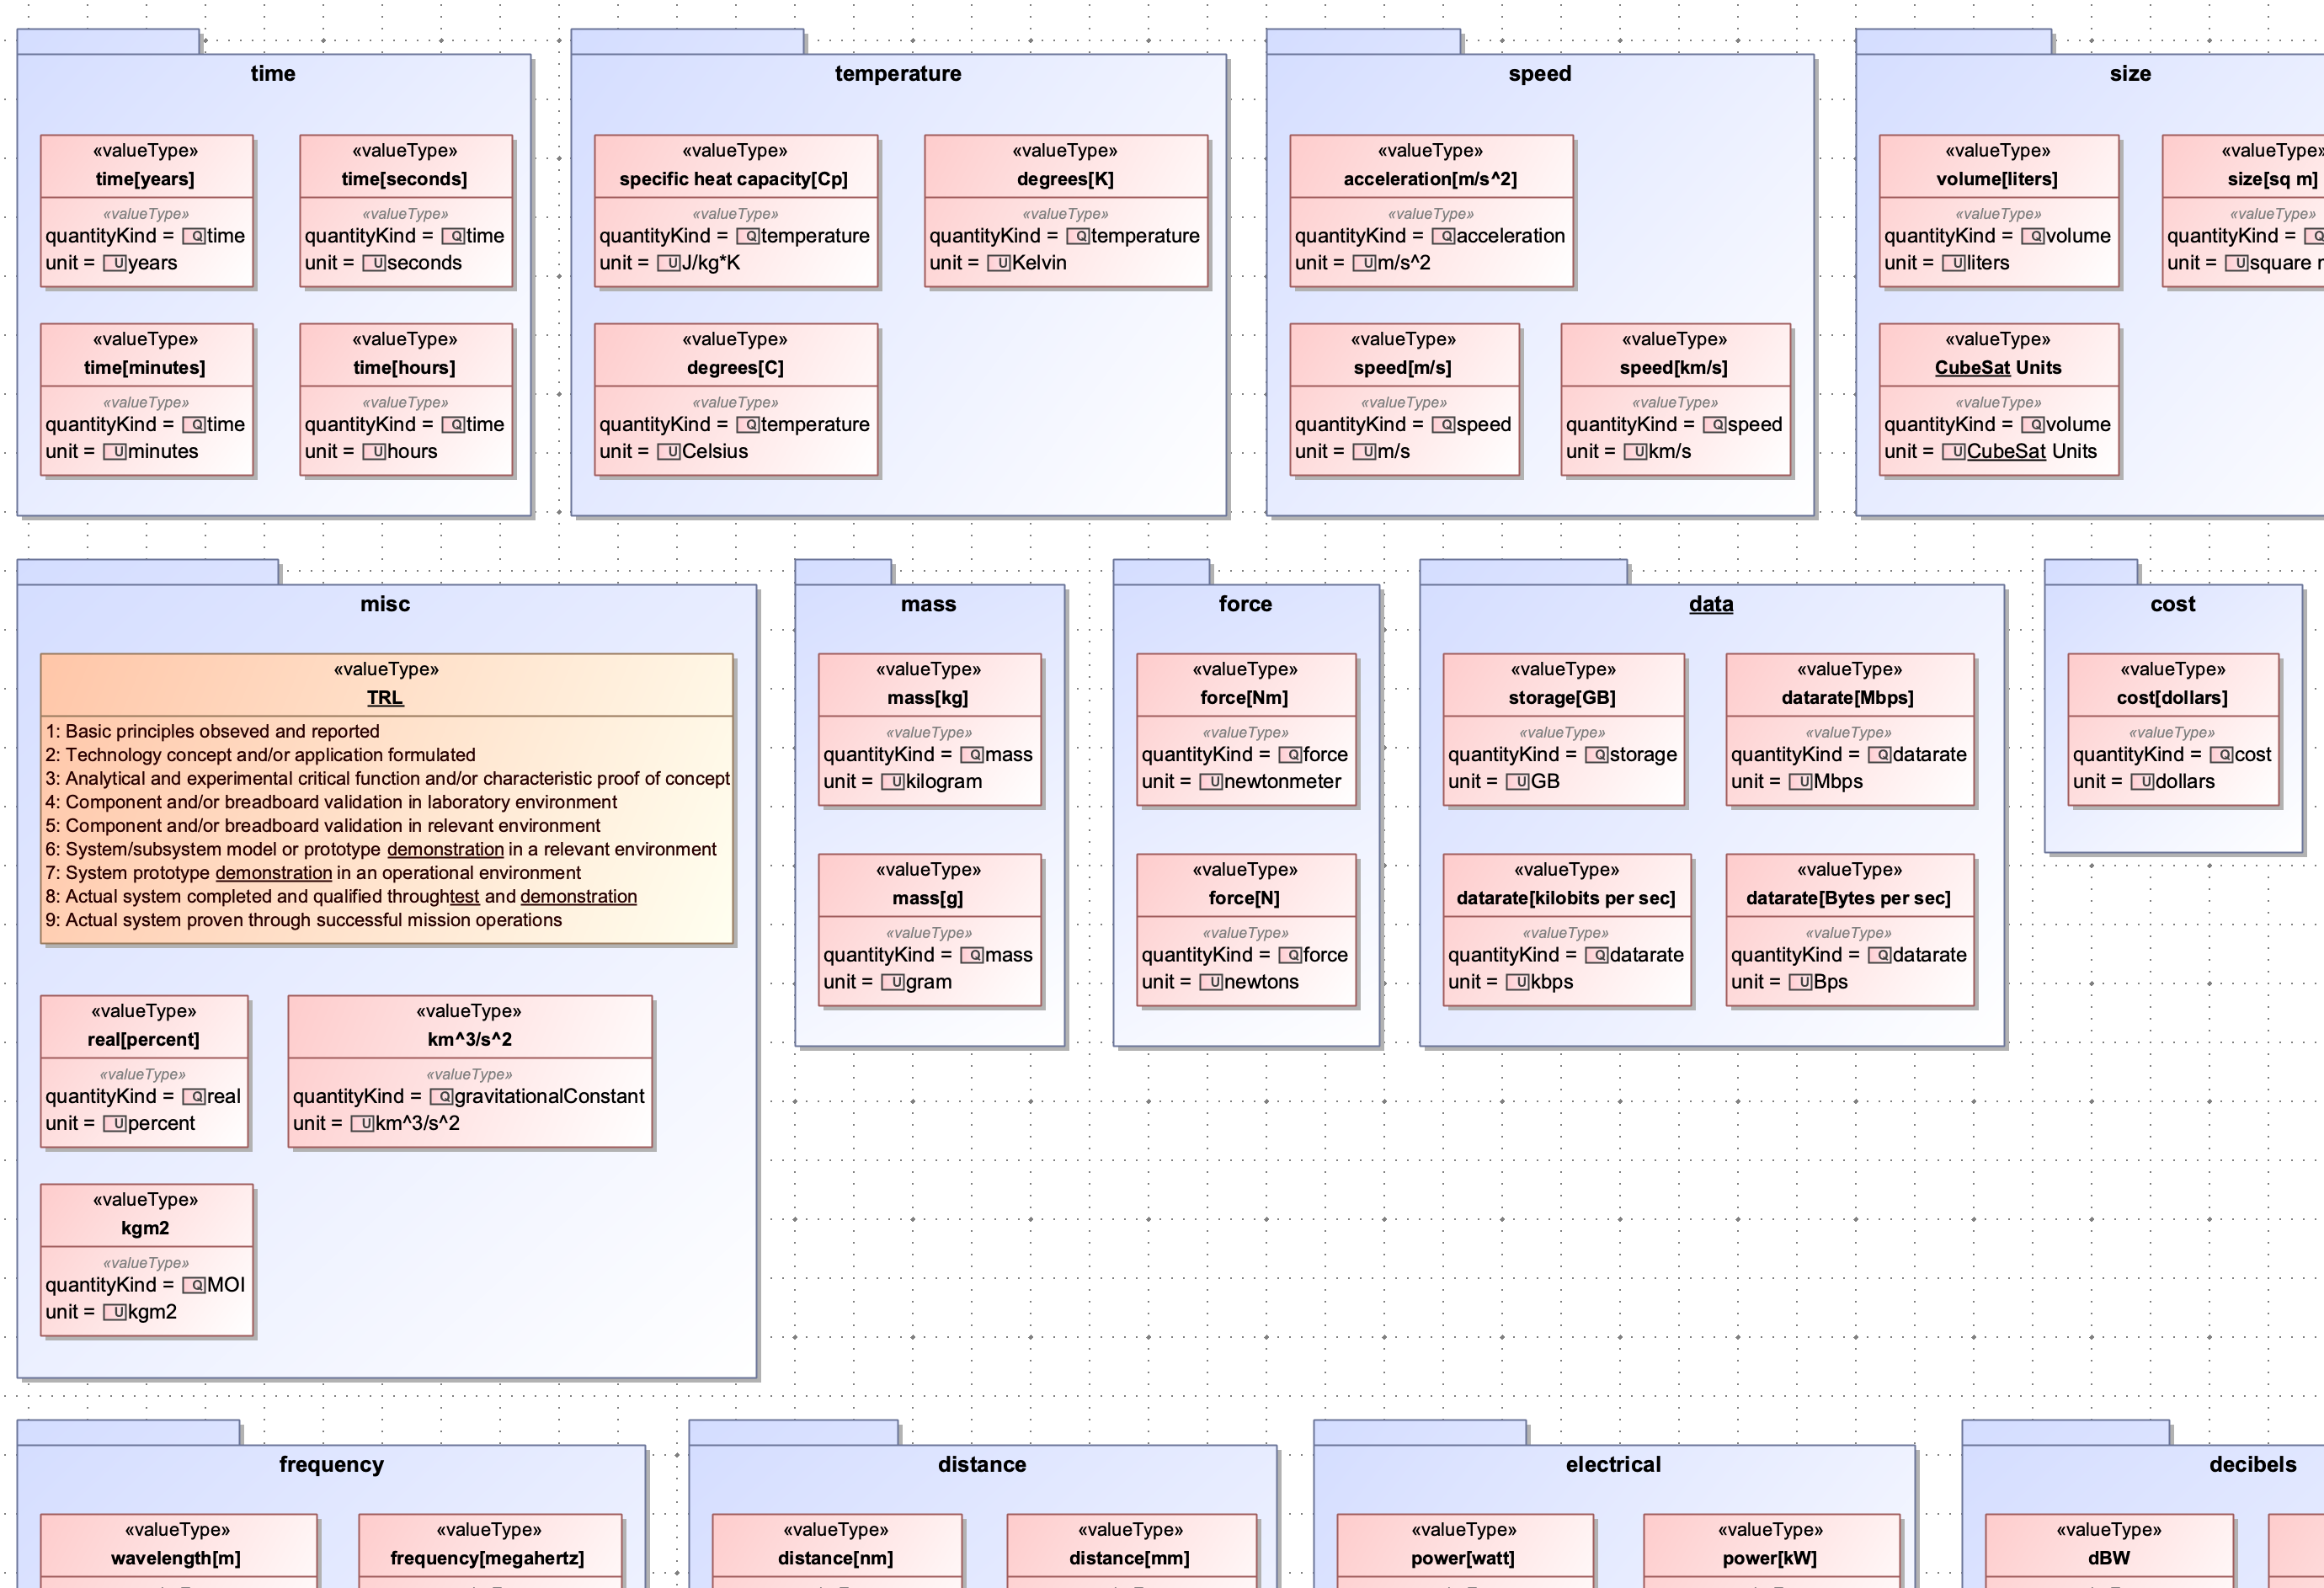
\includegraphics[scale=0.4, angle=90]{Thesis/Analysis_and_Results/Analysis and Results Figures/Value Types.png}
    \caption{Custom Value Type Library}
    \label{fig:Custom Value Type Library}
\end{figure}